\documentclass[a4paper]{article}
\usepackage[utf8]{inputenc}

\usepackage{tikz, sidecap, graphicx}
\usetikzlibrary{positioning, shapes}


\title{Report week 4}
\author{Bård-Kristian Krohg \\ \texttt{baard.krohg@gmail.com}}

\begin{document}
\maketitle

\section{Fitting to model}
My goal this week was to finish this, but I'm still tearing my hair out over it. Mostly, this is due to some rendering issues in rviz. The program runs fast -- at approx. 7.5 - 8 fps. However, the skeleton seems to lag as it updates, and not everything is drawn at once. I shall look into this further.

A couple of things were implemented this week:
\begin{itemize}
\item Accessor functions for the limbs and their attributes.
\item \texttt{'set-'} functions for changing a \texttt{Person} object's keypoints post initialization.
\item Repositioning of keypoints according to fitting the model\footnote{There are still some challenges with this. The results I get seem to compensate too much, and I'm not sure the positions stay updated.}.
\end{itemize}

I also tried to develop a function so only the ``best'' limbs would contribute to scaling the model, but I ended up using a weighted average of all the limbs, as I then didn't need to sort them. The result from this weighted sum was a lot more stable.

In addition, the keypoint positions start to get unpredictable when the subject is too close, $<$500mm, or too far away $>$3000mm. However, the point cloud seems to be fine at these distances, so I'm wondering what's going on.

Next week I want to continue implementing some ideas for refining the 3D position of the keypoints, but I feel I should also try some different approaches I've read about that might yield better results:
\begin{itemize}
\item Using depth points between the two keypoints to estimate a unit vector. (Then place the keypoint along this to the scaled length.) This might be dropped in favor of bulletpoint 3.
\item Improve tracker so I can use previous frames to estimate new position of limbs not observed in the current frame.
\item Compare the accuracy of this manual keypoint allocation with machine learning techniques.
\end{itemize}

\begin{SCfigure}
  \centering
  \caption{The constrained lengths, where we multiply by \emph{scale} to get how the lengths should be proportioned. Based on Drillis R, Contini R. 
\emph{Body Segment Parameters} New York, New York: Office of Vocational 
Rehabilitation; 1966}
  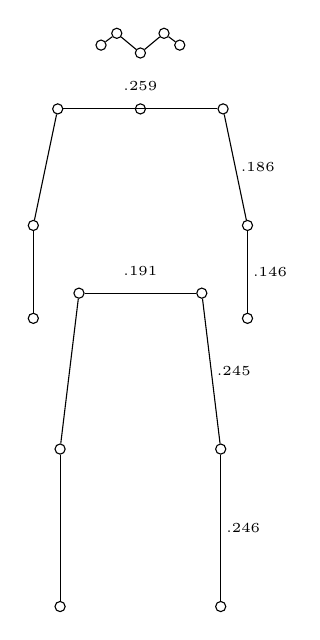
\begin{tikzpicture}[
      every node/.style={draw,circle,minimum size=.06cm, inner sep=1.3pt}
    ]
    \tiny
    %% \draw[help lines, step=5mm, gray!20] (-4,-4) grid (3,4);
    
    \node (nose) at (0,3.25) {};
    \node (neck) at (0,2.54) {};
    
    \node (reye) at (-.3,3.5) {};
    \node (leye) at (.3,3.5) {};

    \node (rear) at (-.5,3.35) {};
    \node (lear) at (.5,3.35) {};

    \node (rshoulder) at (-1.05,2.54) {};
    \node (lshoulder) at (1.05,2.54) {};
    
    \node (relbow) at (-1.36,1.06) {};
    \node (lelbow) at (1.36,1.06) {};

    \node (rwrist) at (-1.36,-.12) {};
    \node (lwrist) at (1.36,-.12) {};

    \node (rhip) at (-.78,.2) {};
    \node (lhip) at (.78,.2) {};

    \node (rknee) at (-1.02,-1.78) {};
    \node (lknee) at (1.02,-1.78) {};

    \node (rankle) at (-1.02,-3.78) {};
    \node (lankle) at (1.02,-3.78) {};

    %% \draw[blue] (0,0) circle [radius=.06cm];

    \draw (reye) -- (nose); \draw (leye) -- (nose);
    \draw (reye) -- (rear); \draw (leye) -- (lear);
    
    \draw (lshoulder) -- node[above, draw=none] {.259} ++(rshoulder);

    \draw (rshoulder) -- (relbow); \draw (lshoulder) -- node[right, draw=none] {.186} ++(lelbow);
    \draw (rwrist) -- (relbow); \draw (lwrist) -- node[right, draw=none] {.146} ++(lelbow);

    \draw (rhip) -- (rknee); \draw (lhip) -- node[right, draw=none] {.245} ++(lknee);
    \draw (rknee) -- (rankle); \draw (lknee) -- node[right, draw=none] {.246} ++(lankle);

    \draw (rhip) -- node[above, draw=none] {.191} ++(lhip);
  \end{tikzpicture}

\end{SCfigure}
\end{document}
